%%%%%%%%%%%%%%%%%%%%%%%%%%%%%%%%%%%%%%%%%
% Masters/Doctoral Thesis 
% LaTeX Template
% Version 2.4 (22/11/16)
%
% This template has been downloaded from:
% http://www.LaTeXTemplates.com
%
% Version 2.x major modifications by:
% Vel (vel@latextemplates.com)
%
% This template is based on a template by:
% Steve Gunn (http://users.ecs.soton.ac.uk/srg/softwaretools/document/templates/)
% Sunil Patel (http://www.sunilpatel.co.uk/thesis-template/)
%
% Template license:
% CC BY-NC-SA 3.0 (http://creativecommons.org/licenses/by-nc-sa/3.0/)
%
%%%%%%%%%%%%%%%%%%%%%%%%%%%%%%%%%%%%%%%%%

%----------------------------------------------------------------------------------------
%	PACKAGES AND OTHER DOCUMENT CONFIGURATIONS
%----------------------------------------------------------------------------------------

\documentclass[
11pt, % The default document font size, options: 10pt, 11pt, 12pt
%oneside, % Two side (alternating margins) for binding by default, uncomment to switch to one side
catalan, % ngerman for German
singlespacing, % Single line spacing, alternatives: onehalfspacing or doublespacing
%draft, % Uncomment to enable draft mode (no pictures, no links, overfull hboxes indicated)
%nolistspacing, % If the document is onehalfspacing or doublespacing, uncomment this to set spacing in lists to single
%liststotoc, % Uncomment to add the list of figures/tables/etc to the table of contents
%toctotoc, % Uncomment to add the main table of contents to the table of contents
%parskip, % Uncomment to add space between paragraphs
%nohyperref, % Uncomment to not load the hyperref package
headsepline, % Uncomment to get a line under the header
%chapterinoneline, % Uncomment to place the chapter title next to the number on one line
%consistentlayout, % Uncomment to change the layout of the declaration, abstract and acknowledgements pages to match the default layout
]{MastersDoctoralThesis} % The class file specifying the document structure

\usepackage[utf8]{inputenc} % Required for inputting international characters
\usepackage[T1]{fontenc} % Output font encoding for international characters
\usepackage{eurosym}
\usepackage{footnote}
\usepackage{palatino} % Use the Palatino font by default
\usepackage{babel}
\usepackage{datetime}
\usepackage[backend=bibtex,natbib=true]{biblatex} % Use the bibtex backend with the authoryear citation style (which resembles APA)
\usepackage{multirow}
\usepackage{float}

\addbibresource{example.bib} % The filename of the bibliography

\usepackage[autostyle=true]{csquotes} % Required to generate language-dependent quotes in the bibliography

%----------------------------------------------------------------------------------------
%	MARGIN SETTINGS
%----------------------------------------------------------------------------------------

\geometry{
	paper=a4paper, % Change to letterpaper for US letter
	inner=2.5cm, % Inner margin
	outer=3.8cm, % Outer margin
	bindingoffset=.5cm, % Binding offset
	top=1.5cm, % Top margin
	bottom=1.5cm, % Bottom margin
	%showframe, % Uncomment to show how the type block is set on the page
}

\newdate{date}{29}{05}{2017}
\date{\displaydate{date}}

%----------------------------------------------------------------------------------------
%	THESIS INFORMATION
%----------------------------------------------------------------------------------------

\thesistitle{Wisebite} % Your thesis title, this is used in the title and abstract, print it elsewhere with \ttitle
\supervisor{Ernest Teniente} % Your supervisor's name, this is used in the title page, print it elsewhere with \supname
\examiner{} % Your examiner's name, this is not currently used anywhere in the template, print it elsewhere with \examname
\degree{Grau en Enginyeria Informàtica} % Your degree name, this is used in the title page and abstract, print it elsewhere with \degreename
\author{Albert Suàrez} % Your name, this is used in the title page and abstract, print it elsewhere with \authorname
\addresses{} % Your address, this is not currently used anywhere in the template, print it elsewhere with \addressname

\keywords{} % Keywords for your thesis, this is not currently used anywhere in the template, print it elsewhere with \keywordnames
\university{\href{http://www.upc.edu}{Universitat Politècnica de Catalunya}} % Your university's name and URL, this is used in the title page and abstract, print it elsewhere with \univname
\department{\href{https://www.essi.upc.edu/}{Departament d'Enginyeria de Serveis i Sistemes d'Informació}} % Your department's name and URL, this is used in the title page and abstract, print it elsewhere with \deptname
\group{\href{https://www.essi.upc.edu/}{ESSI}} % Your research group's name and URL, this is used in the title page, print it elsewhere with \groupname
\faculty{\href{http://www.fib.upc.edu}{Facultat d'Informàtica de Barcelona}} % Your faculty's name and URL, this is used in the title page and abstract, print it elsewhere with \facname

\AtBeginDocument{
\hypersetup{pdftitle=\ttitle} % Set the PDF's title to your title
\hypersetup{pdfauthor=\authorname} % Set the PDF's author to your name
\hypersetup{pdfkeywords=\keywordnames} % Set the PDF's keywords to your keywords
}

\begin{document}

\frontmatter % Use roman page numbering style (i, ii, iii, iv...) for the pre-content pages

\pagestyle{plain} % Default to the plain heading style until the thesis style is called for the body content

%----------------------------------------------------------------------------------------
%	TITLE PAGE
%----------------------------------------------------------------------------------------

\begin{titlepage}
\begin{center}


\includegraphics[scale=0.25]{Figures/logo-upc.png} % University/department logo - uncomment to place it

\vspace*{.06\textheight}
{\scshape\LARGE \univname\par}\vspace{1.5cm} % University name
\textsc{\Large Informe de seguiment}\\[0.5cm] % Thesis type

\HRule \\[0.4cm] % Horizontal line
{\huge \bfseries \ttitle\par}\vspace{0.4cm} % Thesis title
\HRule \\[1.5cm] % Horizontal line
 
\begin{minipage}[t]{0.4\textwidth}
\begin{flushleft} \large
\emph{Autor:}\\
\href{http://www.johnsmith.com}{\authorname} % Author name - remove the \href bracket to remove the link
\end{flushleft}
\end{minipage}
\begin{minipage}[t]{0.4\textwidth}
\begin{flushright} \large
\emph{Director:} \\
\href{http://www.jamessmith.com}{\supname} % Supervisor name - remove the \href bracket to remove the link  
\end{flushright}
\end{minipage}\\[3cm]
 
\vfill

\large \textit{Un treball final de grau corresponent\\ al \degreename}\\[0.3cm] % University requirement text
\textit{en el}\\[0.4cm]
\deptname\\[2cm] % Research group name and department name
 
\vfill

{\large \displaydate{date}}\\[4cm] % Date
 
\vfill
\end{center}
\end{titlepage}

%----------------------------------------------------------------------------------------
%	THESIS CONTENT - CHAPTERS
%----------------------------------------------------------------------------------------

\tableofcontents % Prints the main table of contents

\mainmatter % Begin numeric (1,2,3...) page numbering

\pagestyle{thesis} % Return the page headers back to the "thesis" style

% Include the chapters of the thesis as separate files from the Chapters folder
% Uncomment the lines as you write the chapters

% Chapter 1

\chapter{Introducció} % Main chapter title

\label{Chapter1} % For referencing the chapter elsewhere, use \ref{Chapter1} 

%----------------------------------------------------------------------------------------

% Define some commands to keep the formatting separated from the content 
\newcommand{\keyword}[1]{\textbf{#1}}
\newcommand{\tabhead}[1]{\textbf{#1}}
\newcommand{\code}[1]{\texttt{#1}}
\newcommand{\file}[1]{\texttt{\bfseries#1}}
\newcommand{\option}[1]{\texttt{\itshape#1}}

%----------------------------------------------------------------------------------------

Aquest projecte és un Treball Final de Grau en Enginyeria Informàtica a la Facultat d'Informàtica de Barcelona (\textit{Universitat Politècnica de Catalunya}). Un projecte amb la finalitat principal de convertir un establiment de restauració qualsevol en quelcom intel·ligent, podent gestionar de forma més eficient, còmode i professional les seves comandes, podent-les analitzar posteriorment i interactuant de forma més activa amb el client de l'establiment.

\section{Contextualització}

El món de la restauració va néixer molts segles enrere i amb el transcurs de la història ha anat evolucionant proporcionalment amb l'evolució del ser humà i els seus costums. Tot i així, el que és clar és que el concepte d'anar a prendre quelcom al bar durant algun moment del dia es segueix mantenint per molt temps que passi, almenys a Espanya.
\\\\
La tecnologia ha estat quelcom que sempre ha existit, però no amb tanta importància i impacte com té actualment. Des del naixement de l'\textit{smartphone} \cite{smartphone} el 1992 quan IBM va treure el primer pilot de telèfon mòbil amb funcionalitats de PDA incorporades, s'ha anat instaurant a les nostres vides de manera exponencial fins al punt on és pràcticament una part nostra, que sense ella no seria el mateix. D'aquest aspecte se li pot treure tant punts favorables com negatius. Entre els positius tenim sistemes similars als del projecte que estem tractant, el qual dóna infinitats d'avantatges respecte al sistema convencional. Avui en dia, en el context de la societat actual en què vivim, sistemes intel·ligents implantats en els establiments de restauració es veuen a comptagotes, i no pas perquè les plataformes existents siguin dolentes o precàries, sinó per un altre seguit de factors. Factors com pot ser l'impacte econòmic que implica la instauració d'un sistema d'aquestes característiques, la manca d'adaptabilitat al canvi o bé la complexitat d'alguns establiments.
\\\\
El fet és que des de principis de segle els costums humans canvien amb una rapidesa realment diferent de la de fa segles, tan ràpidament que el món de la restauració en conjunt no s'ha pogut adaptar.
El naixement de les noves tecnologies i el poder que tenen avui en dia a la societat es veu reflectit en bars i restaurants, on algun d'ells (i cada cop més) la utilitzen en el negoci.
Tot i així, en l'estudi d'aquest tòpic, apareix un seguit de qüestions gens menyspreables, les quals han de ser tractades.

\subsection{Factor econòmic}

Un dels principals problemes per als quals aquest sector no s'ha acabat d'adaptar és el cost de la implantació de la tecnologia en un establiment d'aquestes característiques. Cada restaurant o bar és únic en referència a la resta, per tant, cada un d'ells necessita un sistema adaptat a les seves necessitats, i això es fa pagar.
\\\\
El desenvolupament d'un sistema genèric és notablement més barat respecte un específic, ja que l'equip encarregat de construir pot vendre-ho posteriorment a més d'un client, així doncs pot ajustar més el preu. En canvi, si estem parlant d'un sistema totalment personalitzat i especialitzat per un establiment, llavors el cost puja considerablement, ja que han de cobrir els costos del disseny i la implementació del sistema.
\\\\
És aquí doncs on s'estableix un dels tres grans problemes que fa que sistemes d'aquestes característiques no es vegin avui en dia en els establiments de restauració. A més a més se li suma l'època de crisi econòmica viscuda que fa complicar el panorama. Només els establiments que aconsegueixen facturar grans quantitats es poden permetre sistemes com el que comentem.

\subsection{Adaptació al canvi}

En aquest sector ens podem trobar molts tipus d'usuaris. Perfils de gent que sempre busquen ser millors en el sector i fan el possible per estar actualitzats amb la tecnologia d'aquell moment. 
En canvi, existeixen nombrosos casos d'establiments on els responsables d'aquests no tenen facilitat per adaptar-se al canvi, és a dir, que se satisfan amb el procediment de negoci que sempre han tingut i sempre els ha funcionat, encara que sigui antiquat. Amb dificultats com aquestes no és fàcil instaurar un sistema d'aquestes característiques, ja que els usuaris que la utilitzen no s'adaptarien i, en conseqüència, tindria represàlies negatives.
\\\\
La implantació de tot sistema en una corporació o empresa, ja sigui enfocat en el món de la restauració o bé en un altre sector, no només recau en la compra de material \textit{hardware} i \textit{software}, sinó que també recau en la implicació dels treballadors que hauran d'interactuar amb aquest nou sistema. Per tant, és obligació dels responsables de tot establiment que vulgui implantar un sistema d'aquestes característiques motivar a l'equip de treballadors en aquest aspecte. La plataforma a implantar ja pot ser molt bona, però si no hi ha voluntat de l'equip en utilitzar-la correctament, molt probablement el procés acabarà en fallida. 

\newpage
\subsection{Complexitat}

Tots els establiments d'aquest sector funcionen de maneres molt diferents acord a les seves característiques i funcionalitats. Alguns d'ells disposen de sistemes molt complexos i complicats en comparació de la competència, cosa que aporta dificultat en la implantació d'un sistema d'aquest tipus. I en contrapartida, implantar una plataforma d'aquestes característiques en un establiment molt simple com pot arribar a ser un bar de poble tampoc acaba de ser del tot útil.
\\\\
En conseqüència, podem tenir dues situacions que impedeixen el \textit{boom} d'aquests sistemes en el món de restauració. Per una banda, restaurants molt complexos que incapaciten crear un sistema que ho controli tot de forma fàcil. I per altra banda, bars molt simples o senzills que mai s'arribaran a plantejar sistemes d'aquestes característiques.

%----------------------------------------------------------------------------------------

\section{Motivació}

Durant el quadrimestre anterior a l'inici del Treball Final de Grau vaig estar rumiant profundament cap a on volia encaminar el projecte. Tenia disponible la capacitat de realitzar-ho en l'empresa en la qual estava treballant, i actualment segueixo. Tot i així, donades unes circumstàncies que es comentarà a continuació, vaig decidir encaminar-me a realitzar el projecte de \textit{Wisebite}.
\\\\
En el meu context familiar i d'amistats he tingut sempre molt present la cultura de la gastronomia, com bé caracteritza el nostre país. Tot i així, amb els anys he anat coneixent persones que es dediquen professionalment al món de la restauració, sigui cambrers, cuiners o administradors d'establiments del sector. En anar amb aquest tipus de persones a prendre quelcom o a menjar un àpat, em feien veure diferent l'establiment de com ho feia abans. Molts cops ens centràvem més en com era el servei i com estava muntat internament la cadena de producció dins l'establiment que pas gaudir de l'àpat que ens estaven servint.
\\\\
En conseqüència, arran d'això i dels coneixements tècnics que he anat adquirint durant el grau aquests quatre anys, vaig estar pensant com es podria aplicar la tecnologia en establiments d'aquest tipus per tal de millorar la seva eficiència i poder oferir un millor producte als clients.
\\\\
Per dissenyar i construir una idea més autèntica vaig estar parlant amb aquest grup de persones, que s'ha comentat anteriorment, i se'ls va preguntar com funcionaven els seus establiments i que realitzarien per poder millorar-los al que correspon a la gestió del bar o restaurant. Una gran majoria d'aquests em va comentar que van implantar un sistema de gestió de comandes a través d'un mòbil o tauleta, però que els havia costat molt temps acabar-ho implantant donat al cost que comportava. I no només això, sinó que els hi va costar bastant adaptar-se a causa de la poca usabilitat que tenia el sistema que utilitzaven.
\\\\
\newpage
Així doncs, vist quin era l'estat actual, vaig decidir-me a realitzar un estudi de mercat analitzant quines aplicacions i plataformes existien en aquell moment (apartat que comentarem posteriorment) i em vaig adonar que hi havia molta feina per fer. Les aplicacions que aplicaven la filosofia de \textit{Wisebite} estaven bastant obsoletes i no disposaven d'una interfície d'usuari que tendia a la usabilitat, fet que dificultava l'adaptabilitat al canvi dels usuaris.
\\\\
En conclusió, després d'estudiar bé la proposta vaig parlar l'\textit{Ernest Teniente} i va acceptar ser el meu director d'aquest projecte i Treball Final de Grau.
% Chapter Template

\chapter{Estat de l'art} % Main chapter title

\label{Chapter2} % Change X to a consecutive number; for referencing this chapter elsewhere, use \ref{ChapterX}

Per conèixer millor el potencial d'aquest mercat i saber les alternatives per a una major profunditat en el coneixement del sector, s'ha de realitzar un estudi del mercat existent per a comprovar la presència d'aplicacions que són similars, sigui per objectiu o per mercat, a \textit{Wisebite}. A continuació apareixen algunes de les aplicacions que s'han pogut trobar.
\\\\
El fet d'analitzar cadascuna d'elles et permet veure quines funcionalitats pots oferir al client perquè directament no existeix cap eina que les faciliti o bé per millorar les existents. S'ha volgut destacar sis plataformes similars a \textit{Wisebite}, algunes en millors aspectes que altres. En acabar de valorar cadascuna d'elles, es realitzarà un estudi ja més globalitzat que permeti veure quins avantatges ofereix \textit{Wisebite} al mercat actual.

%----------------------------------------------------------------------------------------
%	SECTION 1
%----------------------------------------------------------------------------------------

\section{Waiterio}

Aplicació\cite{waiterio} orientada especialment a substituir el \textit{TPV} d'un bar o restaurant. Disposa de funcionalitats com creació de menús i comandes, convidar companys de feina amb rols associats, visualització en mòbil i tauleta, reports periòdics i generació de factures totals o fraccionades.
\\\\
L'aplicació disposa d'entre unes 50.000 i 100.000 descàrregues al \textit{Play Store}. En general, conté moltes funcionalitats i té una interfície d'usuari ben cuidada que permet l'ús de l'aplicació de forma més còmode i confortable.
\\
\begin{figure}[H]
\centering
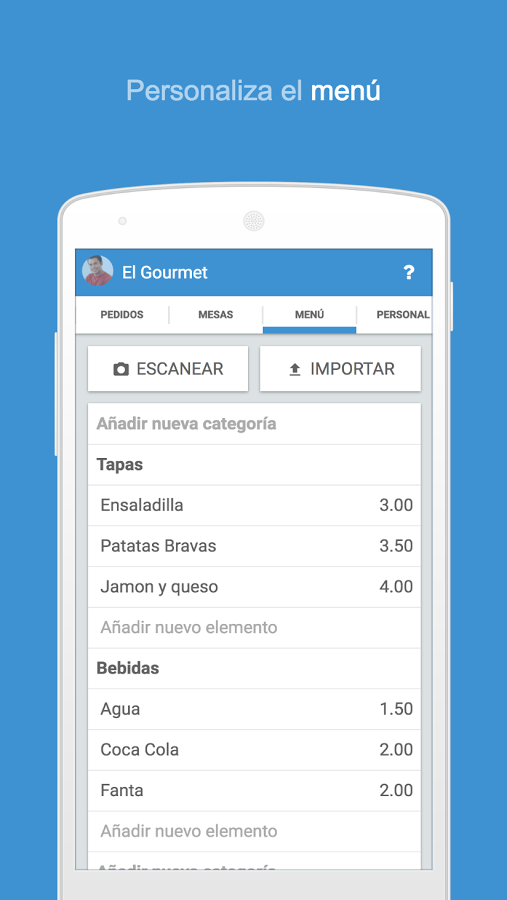
\includegraphics[scale=0.20]{Figures/waitero-1.png}
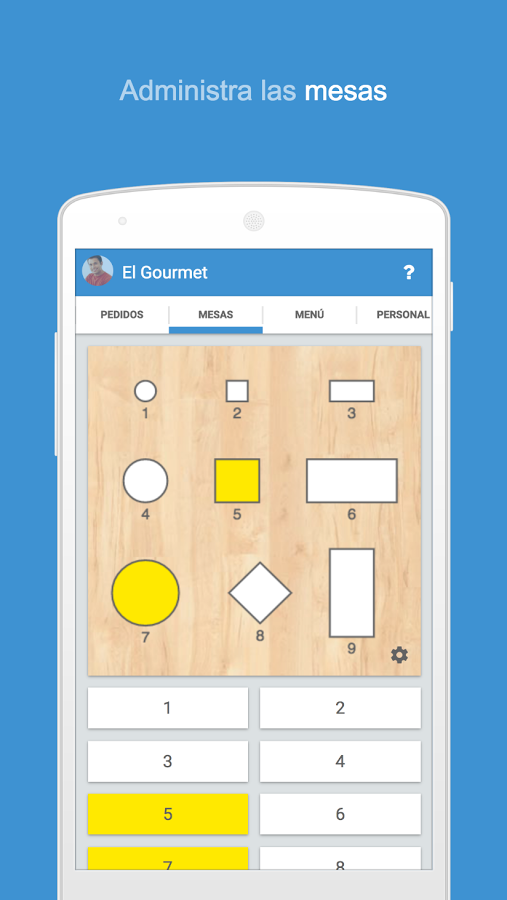
\includegraphics[scale=0.20]{Figures/waitero-2.png}
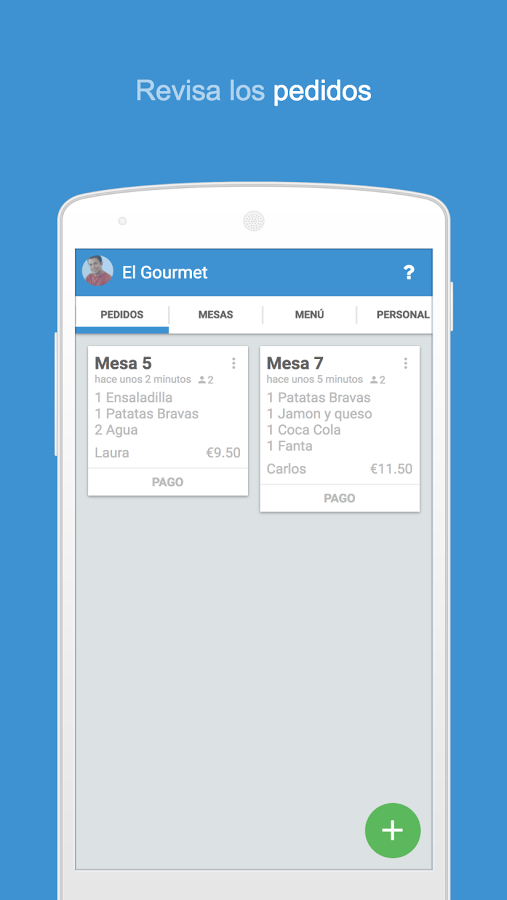
\includegraphics[scale=0.20]{Figures/waitero-3.png}
\caption{Captures de pantalla de Waitero}
\end{figure}



%----------------------------------------------------------------------------------------
%	SECTION 2
%----------------------------------------------------------------------------------------

\section{PrimeTray}

Aplicació\cite{primetray} orientada a les comandes del client a l'establiment. L'usuari té la capacitat de seleccionar un restaurant de la llista i fer la comanda en línia i anar-ho a buscar un cop és notificat. A més a més pot visualitzar l'estat en temps real de la seva comanda, és a dir, si està preparada o encara queda temps per poder-la rebre.
\\\\
L'aplicació té entre 500 i 1.000 descàrregues a la botiga d'aplicacions d'\textit{Android}. Tot i així té un 4.7 de valoració per part dels usuaris. En general l'aplicació està molt ben enfocada pel seu objectiu, és a dir, millorar la comoditat del client en els establiments de restauració als quals acudeix. Té una gestió de la interfície d'usuari prou bona que aconsegueix que sigui més fàcil utilitzar i familiaritzar-se amb l'aplicació. En contrapartida, les funcionalitats d'aquesta aplicació són bastants escasses. Fet que aconsegueix que perdi molts punts en comparació altres empreses.
\\
\begin{figure}[H]
\centering
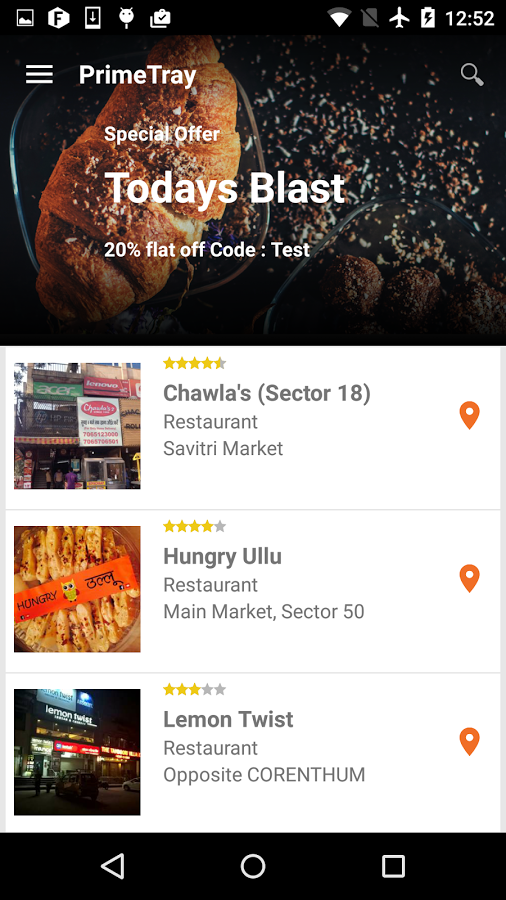
\includegraphics[scale=0.20]{Figures/primetray-1.png}
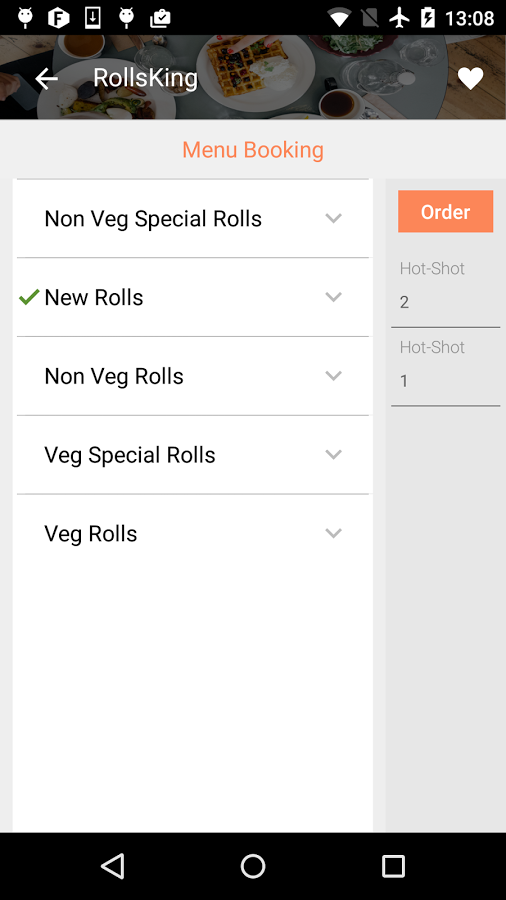
\includegraphics[scale=0.20]{Figures/primetray-2.png}
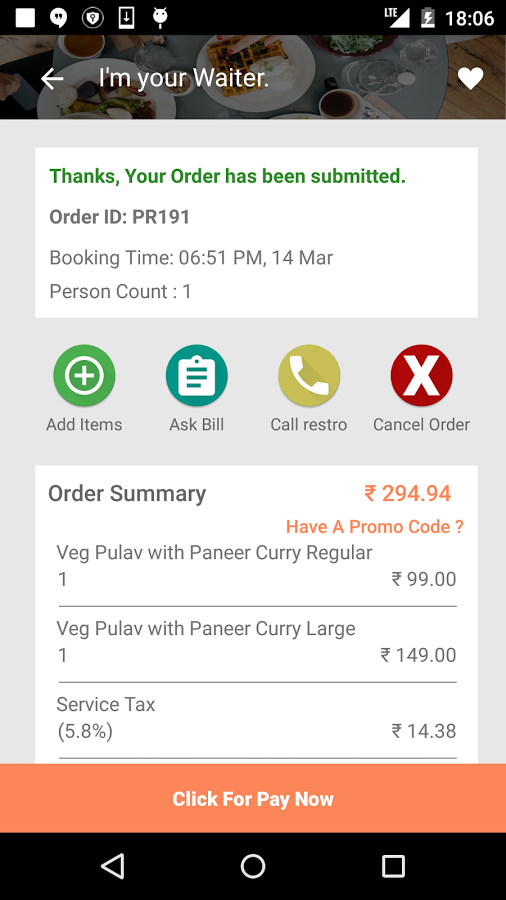
\includegraphics[scale=0.20]{Figures/primetray-3.png}
\caption{Captures de pantalla de PrimeTray}
\end{figure}

%----------------------------------------------------------------------------------------
%	SECTION 3
%----------------------------------------------------------------------------------------

\section{OrderSev}

Aplicació\cite{ordersev} orientada especialment a substituir el \textit{TPV} d'un bar o restaurant. Disposa de funcionalitats com creació de menús i comandes, generació de factures i vistes tant des de cuina com del cambrer. Gran punt a favor que disposa aquesta aplicació és la vista web de la qual disposa. Pots accedir de forma multiplataforma segons l'objectiu que tens amb l'aplicació.
\\\\
Disposa d'entre 500 i 1.000 descàrregues, i amb una nota mitjana de 5.0, però amb només 17 votacions, ha acabat sent una aplicació funcional però amb no gaire repercussió. El punt en contra que és que no li han dedicat el temps en la interfície d'usuari que comporta. Disposa d'unes vistes molt simples i molt poc estètiques.
\\\\
La gestió de la interfície d'usuari és quelcom molt important a l'hora de valorar una aplicació. Pel simple fet que els usuaris que la utilitzin no es fixaran en si l'algorisme i les tecnologies utilitzades són molt bones o no, sinó en quin aspecte té l'aplicació. És per això doncs que aquesta aplicació no ha acabat de triomfar, pel simple fet que la interfície no era l'adequada pel tipus d'usuari amb el qual treballava.
\\
\begin{figure}[H]
\centering
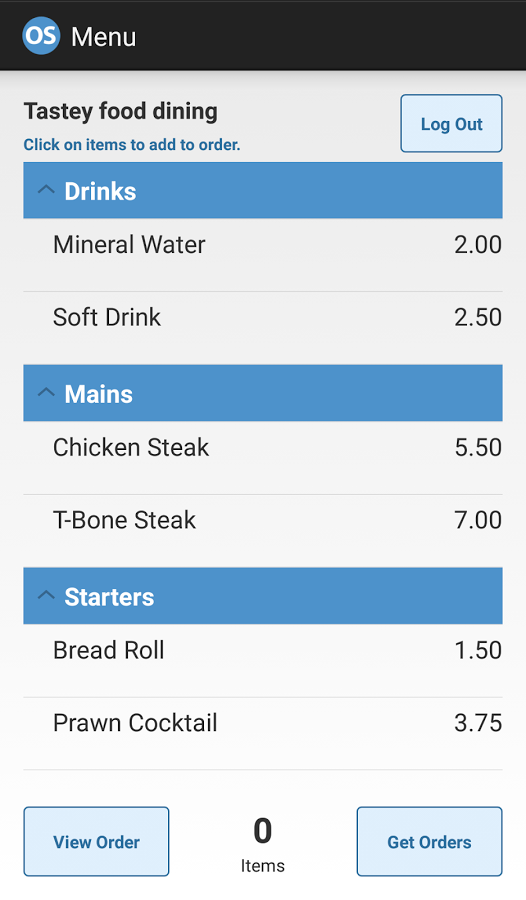
\includegraphics[scale=0.20]{Figures/ordersev-1.png}
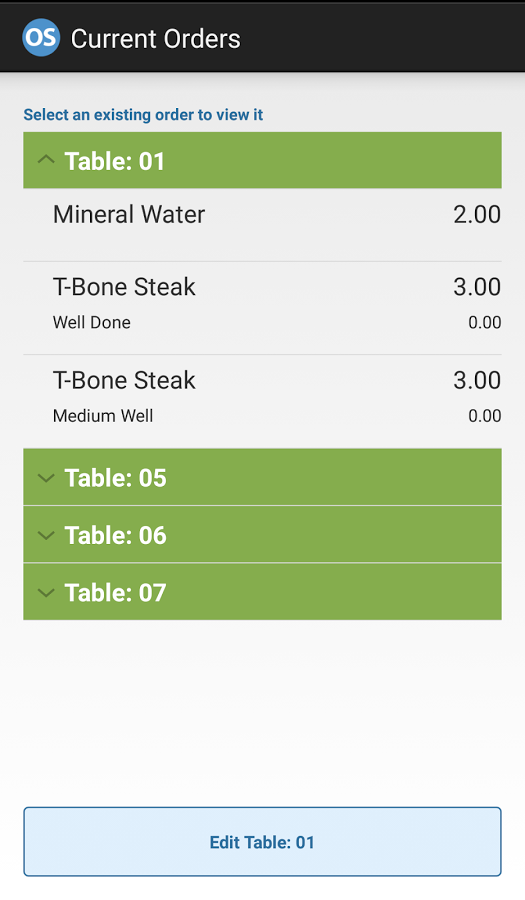
\includegraphics[scale=0.20]{Figures/ordersev-2.png}
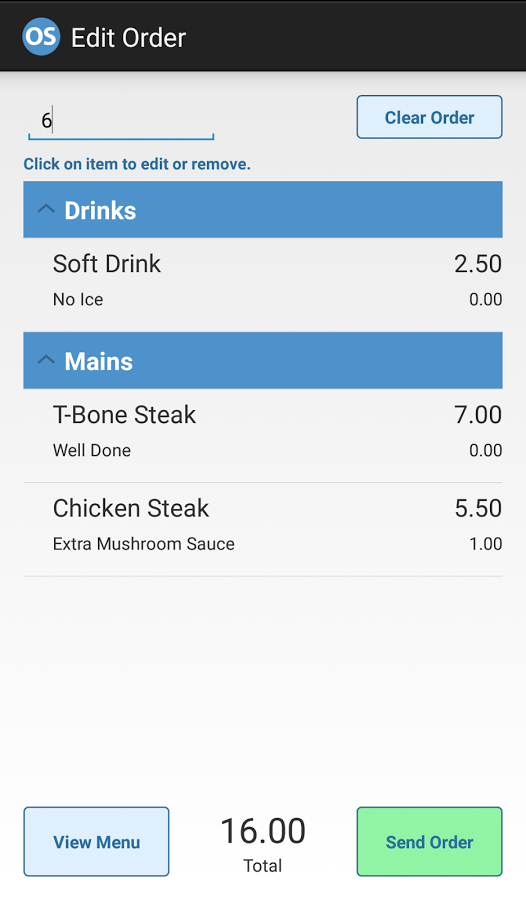
\includegraphics[scale=0.20]{Figures/ordersev-3.png}
\caption{Captures de pantalla de OrderSev}
\end{figure}

%----------------------------------------------------------------------------------------
%	SECTION 4
%----------------------------------------------------------------------------------------

\section{TabletWaiter}

Aplicació\cite{tabletwaiter} orientada a ser un estil de carta per a l'establiment. Cada taula d'un restaurant hauria d'haver-hi un dispositiu amb aquesta aplicació activa a on es pugui consultar els plats i seleccionar-los, així es rebria a cuina i ja podrien començar a preparar la comanda. També permet cridar al cambrer via aplicació i demanar el compte. Per altra banda, també disposa de la possibilitat que un cambrer la utilitzi per crear la comanda. És a dir, l'aplicació està preparada per ambdós perfils, ja sigui client com cambrer. Permet accedir-hi en la seva versió web, a on es pot crear els menús i parametritzar com vulguis el teu bar o restaurant.
\\\\
Aquesta aplicació, amb un conjunt de descàrregues situat entre 1.000 i 5.000 i un valor de 3.7 com a puntuació dels usuaris, es situa en un bon lloc en el mercat donat les funcionalitats que disposa. Tot i així, no ha acabat mai de despuntar a causa de la seva gestió de la interfície d'usuari. Les aplicacions per a dispositius mòbils han anat evolucionant en el que el seu disseny es refereix cap a un punt on totes les plataformes segueixen els mateixos patrons de disseny, patrons com \textit{Material Design}\cite{materialdesign}. Fet que no aplica aquesta aplicació. La plataforma disposa d'una interfície que no aplica cap tipus de patró de disseny, fet que dificulta la usabilitat de l'usuari.
\\
\begin{figure}[H]
\centering
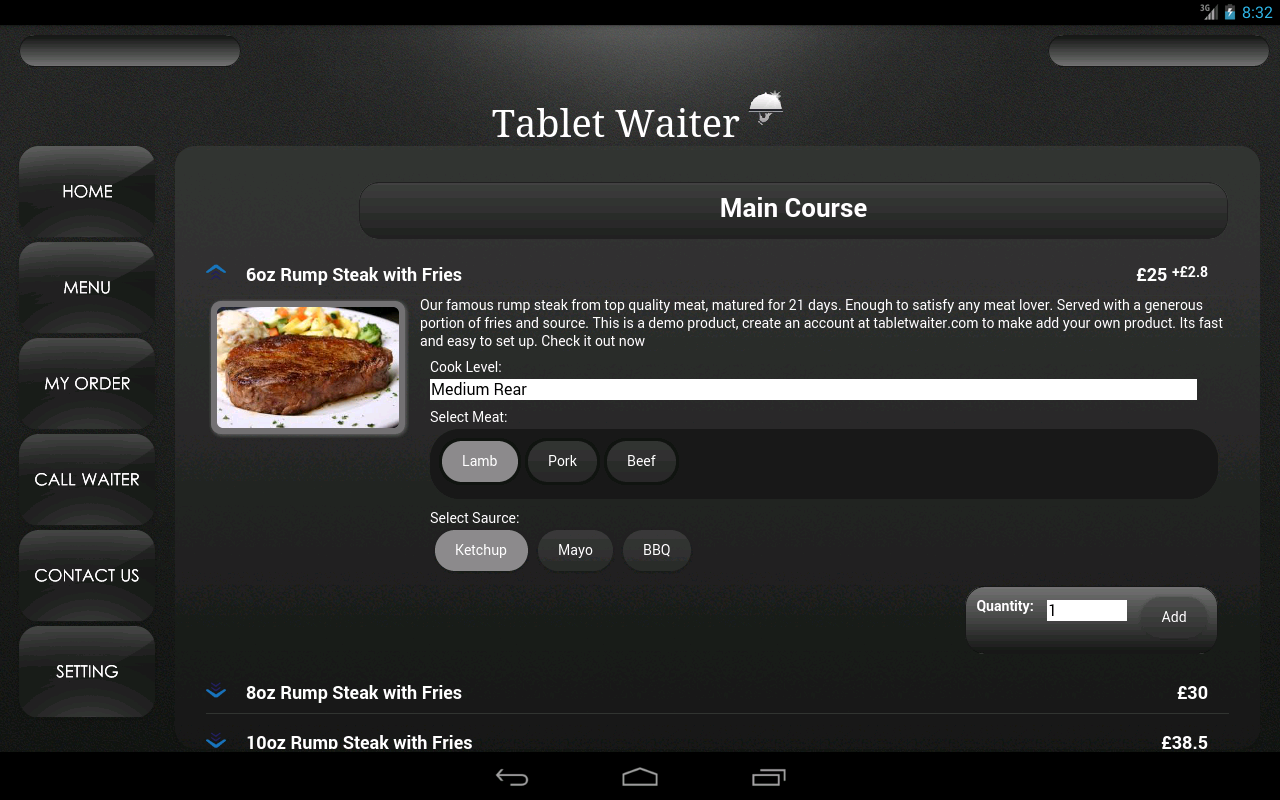
\includegraphics[scale=0.15]{Figures/tabletwaiter-1.png}
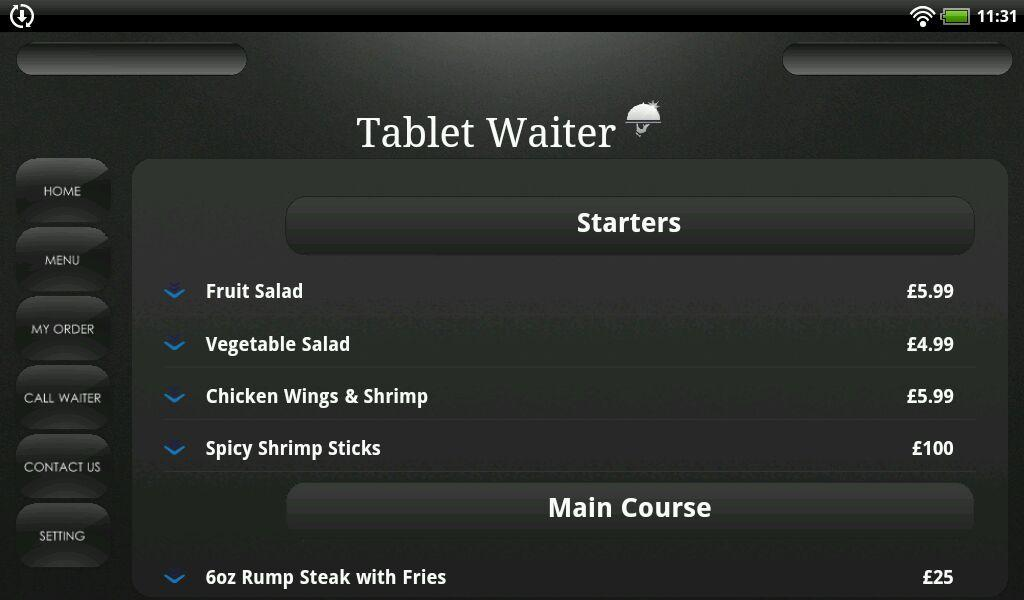
\includegraphics[scale=0.20]{Figures/tabletwaiter-2.png}
\caption{Captures de pantalla de TabletWaiter}
\end{figure}

%----------------------------------------------------------------------------------------
%	SECTION 5
%----------------------------------------------------------------------------------------

\newpage
\section{Cloud Waiter}

Aplicació\cite{cloudwaiter} orientada a les comandes del client a l'establiment. L'usuari té la capacitat d'escanejar un codi QR amb el qual podrà accedir a l'aplicació i realitzar la comanda. Així doncs l'usuari client que acudeix a l'establiment podrà estar-hi el temps que vegi precís i podrà demanar el que vulgui sense necessitat d'esperar al cambrer que l'assisteixi. A part, també disposa de la funcionalitat de poder cridar al cambrer perquè s'acosti a la taula tant per consultes com per demanar el compte.
\\\\
Plataforma amb un volum de descàrregues d'entre 1.000 i 5.000 i una valoració de 4.6 sobre 5 per part dels usuaris, es converteix en una aplicació bastant correcta en l'àmbit en el qual s'especialitza, és a dir, millorar l'experiència del client en l'establiment. Malauradament aquesta aplicació no ha acabat de sortir a la llum pel mateix problema que s'ha comentat en l'aplicació anterior, o sigui, la dolenta gestió d'interfície d'usuari.
\\
\begin{figure}[H]
\centering
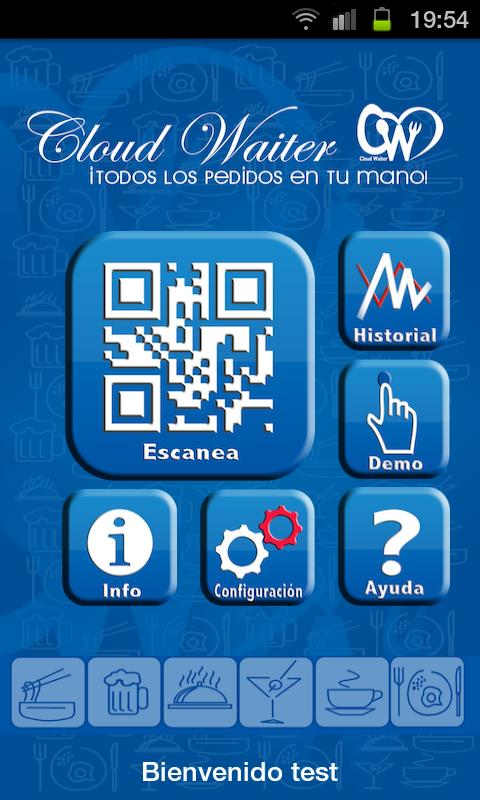
\includegraphics[scale=0.20]{Figures/cloudwaiter-1.jpg}
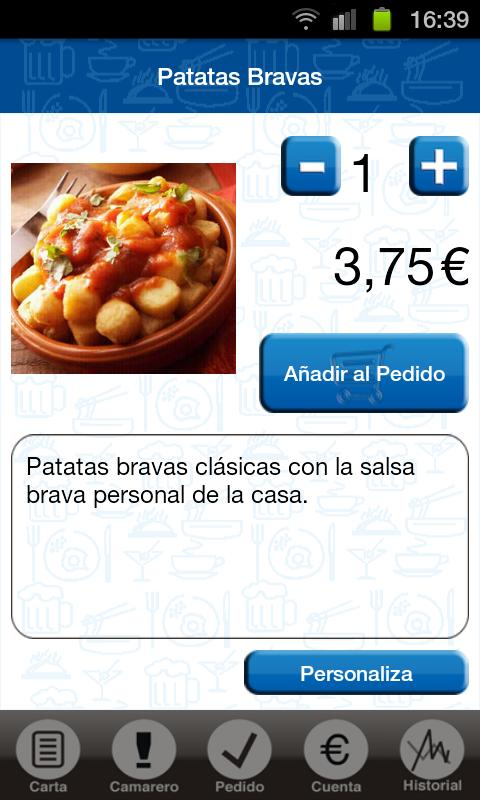
\includegraphics[scale=0.20]{Figures/cloudwaiter-2.jpg}
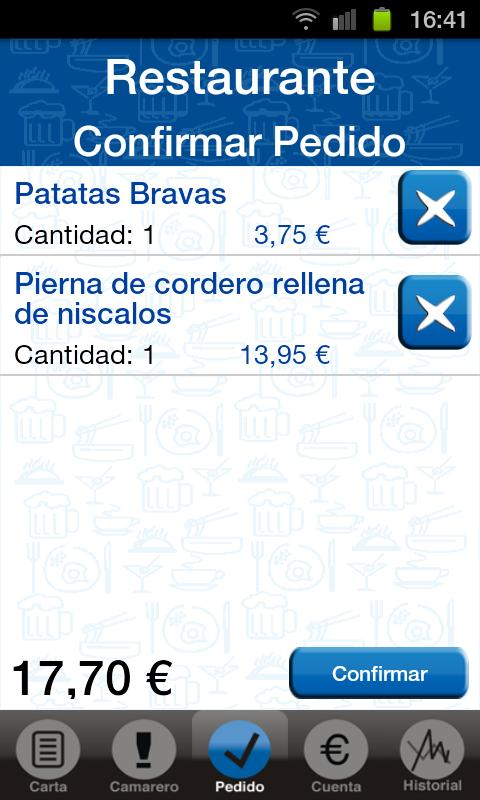
\includegraphics[scale=0.20]{Figures/cloudwaiter-3.jpg}
\caption{Captures de pantalla de OrderSev}
\end{figure}

%----------------------------------------------------------------------------------------
%	SECTION 6
%----------------------------------------------------------------------------------------

\section{FastOrder}

Aplicació\cite{fastorder} orientada a les comandes del client a l'establiment. L'usuari té la capacitat d'escanejar un codi QR amb el qual podrà accedir a l'aplicació i realitzar la comanda i tot el que sigui necessari. Diferents usuaris poden accedir a la mateixa comanda i modificar-la segons vegin convenient, fet que permet que cadascun dels clients d'una mateixa taula puguin fer la comanda de forma paral·lela.
\\\\
Aplicació amb més de 5.000 però amb menys de 10.000 descàrregues i amb una valoració de 4.7 per part de la comunitat d'usuaris, es situa amb una de les que disposa de més usuaris en comparació de les que s'han comparat. Aquesta plataforma disposa de funcionalitats un xic limitades en comparació de la competència, però en contrapartida té una interfície d'usuari molt ben cuidada. Fet que la permès situar-se amb el nombre de descàrregues que disposa actualment.
\\
\begin{figure}[H]
\centering
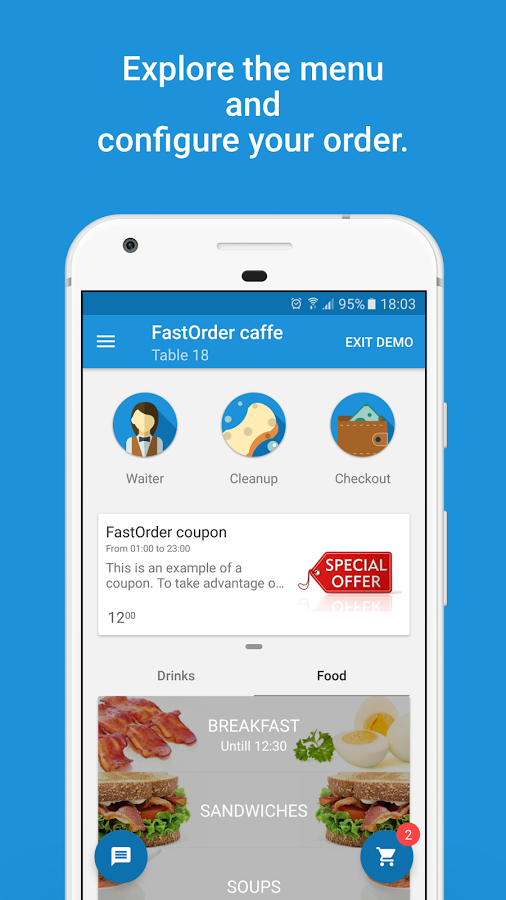
\includegraphics[scale=0.20]{Figures/fastorder-1.png}
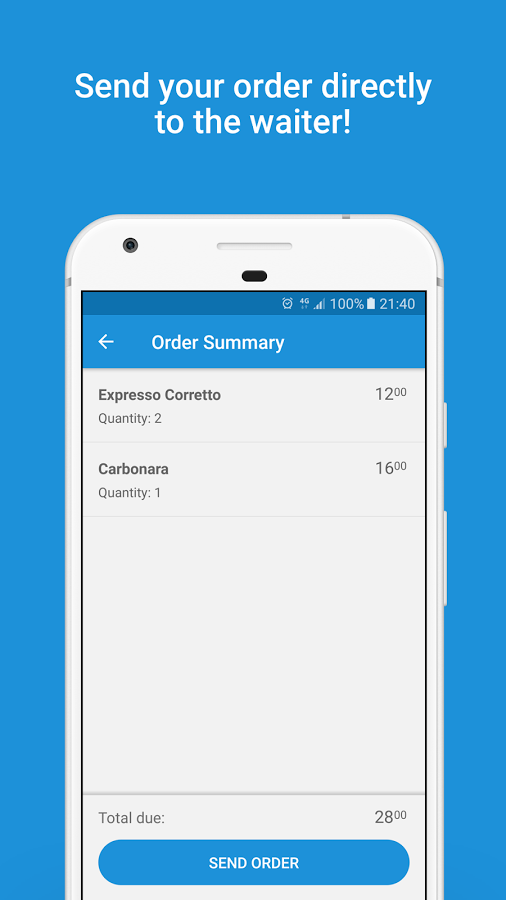
\includegraphics[scale=0.20]{Figures/fastorder-2.png}
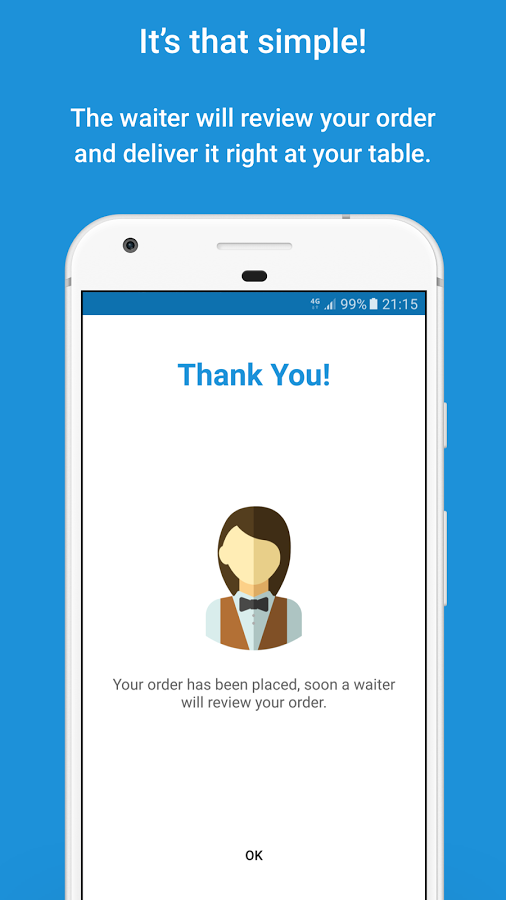
\includegraphics[scale=0.20]{Figures/fastorder-3.png}
\caption{Captures de pantalla de OrderSev}
\end{figure}

%----------------------------------------------------------------------------------------
%	SECTION 7
%----------------------------------------------------------------------------------------

\section{Conclusions}

Encara que hi ha moltes aplicacions relacionades amb aquest àmbit (si bé, amb objectius i funcionalitats molt diverses, en alguns casos molt dispars al projecte), s'ha fet una selecció prou representativa però tot i així reduïda, amb l'objectiu de realitzar una correcta anàlisi que permeti treure conclusions de forma còmoda i eficaç.
\\\\
Un cop realitzada aquesta selecció de potencials competidors de l'aplicació, i comprès (a grans trets) les seves funcionalitats i objectius, procedim a un estudi detallat comparant-ho amb la visió d'aquest projecte.
\\\\
El que s'ha pogut veure estudiant el mercat és que hi ha dos grans grups d'aplicacions. Per una banda, tenim els sistemes que només se centren en la gestió interna de l'establiment i poder realitzar comandes més fàcil i eficientment. Per altra banda, tenim les plataformes que permeten al client, que acudeix a l'establiment, viure una millor experiència i estar còmode en la seva estança. Resumint, hi ha aplicacions que milloren a l'empleat de l'establiment i altres que aporten comoditat al client.
\\\\
Altre punt realment important, i que s'ha pogut demostrar en l'anàlisi de cada una de les aplicacions anteriors, és la gestió de la interfície d'usuari (\textit{GUI}). Gran part dels usuaris que podrien arribar a utilitzar aquest tipus d'aplicacions o plataformes són usuaris no especialitzats en la tecnologia, també coneguts per l'anglicisme \textit{laypeople}. En conseqüència, és realment vital centrar-se a construir una bona experiència d'usuari i dissenyar una aplicació que sigui fàcil d'utilitzar, intuïtiva i fàcil d'aprendre per qualsevol tipus de perfil d'usuari. Un exemple podria ser \textit{FastOrder}, una aplicació que escasseja clarament de funcionalitats si ho comparem amb la resta d'aplicacions del mercat, però en canvi es situa la segona amb més descàrregues dins del \textit{Play Store}. Per què? Perquè al cap i a la fi el primer impacte que reps d'una aplicació, sigui mòbil o web, és la interfície d'aquesta. Si la plataforma disposa d'una bona experiència per l'usuari, aquest la seguirà utilitzant de forma genèrica i fins i tot l'acabarà recomanant al seu cercle.
\\\\
En conclusió, un cop estudiat quin és el mercat, es veu clar quina és la tendència i que pot aportar \textit{Wisebite} a aquest sector.
\\\\
Per un cantó, les nombroses funcionalitats que disposen les aplicacions comentades es podrien agrupar en tres grans grups: gestió de l'establiment, anàlisi de dades i relació amb el client. El primer d'ells es basa en tot el que engloba la digitalització de l'establiment, el segon és l'explotació de les dades digitalitzades per a la millora en l'eficiència i gestió del bar o el restaurant i per últim la millora en l'experiència del client en l'establiment. El fet és que no existeix cap plataforma que implanti les tres funcionalitats, com a molt dues d'elles. \textit{Wisebite} té la intenció d'adaptar les tres en una sola plataforma, i no només això, sinó millorar les prestacions de cada un d'elles.
\\\\
Per altra banda, i com ja s'ha comentat en estudiar cada un dels exemples anteriors, \textit{Wisebite} té molt a aportar en el que la gestió de la interfície d'usuari es tracta. No només es vol disposar d'un sistema òptim des d'un sentit computacional, sinó tenir una interfície d'usuari usable, intuïtiva i comprensible per qualsevol tipus de client, sobretot fent èmfasi en el sector \textit{laypeople}.
\\\\
Així doncs, \textit{Wisebite} aportarà un nou estil d'aplicació desconegut en el sector fins al dia d'avui que facilitarà el dia a dia a tota persona relacionada, ja sigui client com empleat.
% Chapter Template

\chapter{Planificació} % Main chapter title

\label{Chapter3} % Change X to a consecutive number; for referencing this chapter elsewhere, use \ref{ChapterX}

En la primera fase del projecte es va realitzar una planificació inicial a on s'especificava quines tasques en realitzarien durant el Treball Final de Grau, com s'organitzarien i, sobretot, quan temps es dedicaria en cada una d'elles. Després d'haver transcorregut tres mesos dels quatre que aproximadament dura el projecte, hi ha hagut punts que es van estimar correctament i s'han pogut dur a terme sense cap tipus de problemàtica però d'altres que s'han vist forçats a modificar. Un cop analitzats es veurà si finalment, fent balanç, ha modificat l'objectiu final de projecte.

\section{Acord amb la planificació inicial}

En el seu moment es va definir una metodologia de treball inspirada en la metodologia àgil Scrum, amb un seguit de cinc sprints o iteracions a on es desenvoluparia la implementació del projecte. L'objectiu era definir un \textit{backlog} inicial amb totes les \textit{històries d'usuari} que contindria el projecte i, en cada un dels \textit{sprint plannings}, atribuir un conjunt d'aquestes a aquell sprint.
\\\\
Després d'aquests tres mesos de projecte es pot dir que s'ha seguit aquest patró o metodologia de treball. A més a més, comentar que la durada de les dues setmanes per iteració que es va atribuir a la planificació inicial s'ha respectat amb una variació màxima de 2 o 3 dies.


\section{Modificacions}

El canvi més important que s'ha realitzat acord amb la planificació inicial del projecte, però que no modifica el fet d'arribar a l'objectiu final en el temps acordat, és l'alteració en l'ordre de les tasques. En el seu moment es va estipular la idea de realitzar durant dos mesos tota la implementació del projecte i, en l'ultim més, redactar la memòria documentant tota la implementació realitzada durant la fase intermèdia.
\\\\
El canvi ha estat degut per un seguit de factors. Tant el director del projecte com l'alumne que el porta a càrrec es van adonar que realitzar l'ordre de tasques estipulat inicialment portaria a la problemàtica de no tenir una bona documentació final a entregar. En primer lloc pel poc temps que es disposava en comparació del que es necessita per realitzar una bona memòria, i per altra banda el fet de documentar tot al final podria donar lloc a no realitzar una documentació de la implantació del tot acurada donat el temps entre finalitzar el codi i explicar-lo. A més a més, el fet d'anar intercalant implementació amb documentació faria més amè el transcurs del projecte.
\\\\
Per altra banda, hi ha hagut modificacions en la implementació de les \textit{històries d'usuari}. Inicialment, al realitzar i definir \textit{backlog} inicial, es van crear un seguit de \textit{features} sense contemplar del tot el temps que es disposava per implementar-les. Llavors, durant la realització de la iteració, l'alumne es va adonar que aquestes històries d'usuari aportaven un esforç extra en l'sprint que no es veia reflectit en el resultat final. És a dir, l'esforç que es necessitava per implementar aquestes històries d'usuari no era equivalent al valor que aportava a l'usuari final del producte. En conseqüència, per tal de solucionar aquesta problemàtica, es va decidir presidir d'aquestes \textit{features} donat el temps acotat del projecte.


\section{Conclusions}

Finalment, es pot considerar que tot i les modificacions respecte la planificació inicial, no hi haurà cap problemàtica en arribar de forma correcte al \textit{deadline} del projecte. Actualment ja s'ha implementat la primera fase del treball, corresponent a tota història d'usuari referent a la gestió del restaurant, la qual representa més del 60\% del treball.
\\\\
Paral·lelament ja s'ha documentat bona part de la memòria, concretament s'han redactat de forma definitiva els tres primers capítols corresponents a la contextualització, motivació, estat de l'art, objectius, abast, obstacles i metodologia. I a més s'ha començat a redactar altres punts com els agents implicats, tecnologies utilitzades, planificació, gestió econòmica i sostenibilitat.
% Chapter Template

\chapter{Metodologia} % Main chapter title

\label{Chapter4} % Change X to a consecutive number; for referencing this chapter elsewhere, use \ref{ChapterX}

Inicialment es va planificar utilitzar i dur a terme una metodologia àgil inspirada en \textit{Scrum}, és a dir, definir sprints o iteracions amb un conjunt d'històries d'usuari o \textit{features} en el seu interior, les quals estarien ponderades amb un cost X per tal de poder-les prioritzar amb més facilitat. Com s'ha comentat al capítol anterior, es van definir cinc iteracions de dues setmanes cadascuna a on s'implementava el projecte a realitzar.
\\\\
Després d'estar aplicant aquesta metodologia durant els pràcticament dos mesos que està durant la fase intermèdia del projecte, es pot considerar que es va prendre una bona decisió utilitzant-la i s'ha mantingut i es mantindrà durant tot el transcurs del treball.
% Chapter Template

\chapter{Identificació de lleis i regulacions} % Main chapter title

\label{Chapter5} % Change X to a consecutive number; for referencing this chapter elsewhere, use \ref{ChapterX}

Aquest projecte no utilitza cap tipus de dades d'alguna font externa, en conseqüència, no disposa de cap problemàtica referent al \textit{copyright}\cite{copyright} en aquest aspecte. Tot i així, s'han tingut alguns factors a l'hora de decidir quines tecnologies i media utilitzar.
\\\\
Durant el transcurs de la implementació del projecte s'ha prioritzat sempre l'ús de tecnologies \textit{OpenSource}\cite{opensource} i de Software Lliure abans que tecnologies d'ús privatiu. Malauradament, hi ha hagut punts on no s'ha pogut realitzar i s'ha acabat decantant per l'ús de tecnologies \textit{freeware}\cite{freeware}. A la vegada, quan es requeria alguna imatge o audiovisual a adjuntar en la documentació o dins l'aplicació, s'ha prioritzat també l'ús d'imatges \textit{copyleft}\cite{copyleft}, és a dir, amb drets de reutilització per part de l'autor del projecte.

\cleardoublepage
% \phantomsection
\addcontentsline{toc}{chapter}{\listfigurename}
\listoffigures % Prints the list of figures

%----------------------------------------------------------------------------------------
%	ABBREVIATIONS
%----------------------------------------------------------------------------------------

\cleardoublepage
% \phantomsection
\addcontentsline{toc}{chapter}{Índex d'abreviacions}
\begin{abbreviations}{ll} % Include a list of abbreviations (a table of two columns)

\textbf{IBM} & \textbf{I}nternational \textbf{B}usiness \textbf{M}achines\\
\textbf{PDA} & \textbf{P}ersonal \textbf{D}igital \textbf{A}ssistant\\
\textbf{TPV} & \textbf{T}erminal \textbf{P}unt de \textbf{V}enda\\
\textbf{GUI} & \textbf{G}raphical \textbf{U}ser de \textbf{I}nterface\\

\end{abbreviations}

%----------------------------------------------------------------------------------------
%	BIBLIOGRAPHY
%----------------------------------------------------------------------------------------

\printbibliography[heading=bibintoc]

%----------------------------------------------------------------------------------------

\end{document}  